\chapter*{Anexo I: Guía de uso}\label{Anexo}
\pagestyle{especial}
\chaptermark{Anexo I: Guía de uso}
\phantomsection
\addcontentsline{toc}{listasf}{Anexo I: Guía de uso}

\section{Descripción y cuadro de mandos}

En este panel de control (figura \ref{fig:interfazhmireal}) se pueden encontrar los siguientes elementos:

\begin{itemize}
    \item Pantalla LCD.
    \item Seta de Emerencia.
    \item Interruptor de selección modo LOCAL/REMOTO.
    \item INterruptor de selección modo MICRO/SIN MICROCONTROLADOR.
    \item Botón de flechas de selección del menú.
    \item Botón ENTER.
    \item Botón Escape
\end{itemize}

\begin{figure}[htbp]
	\centering
	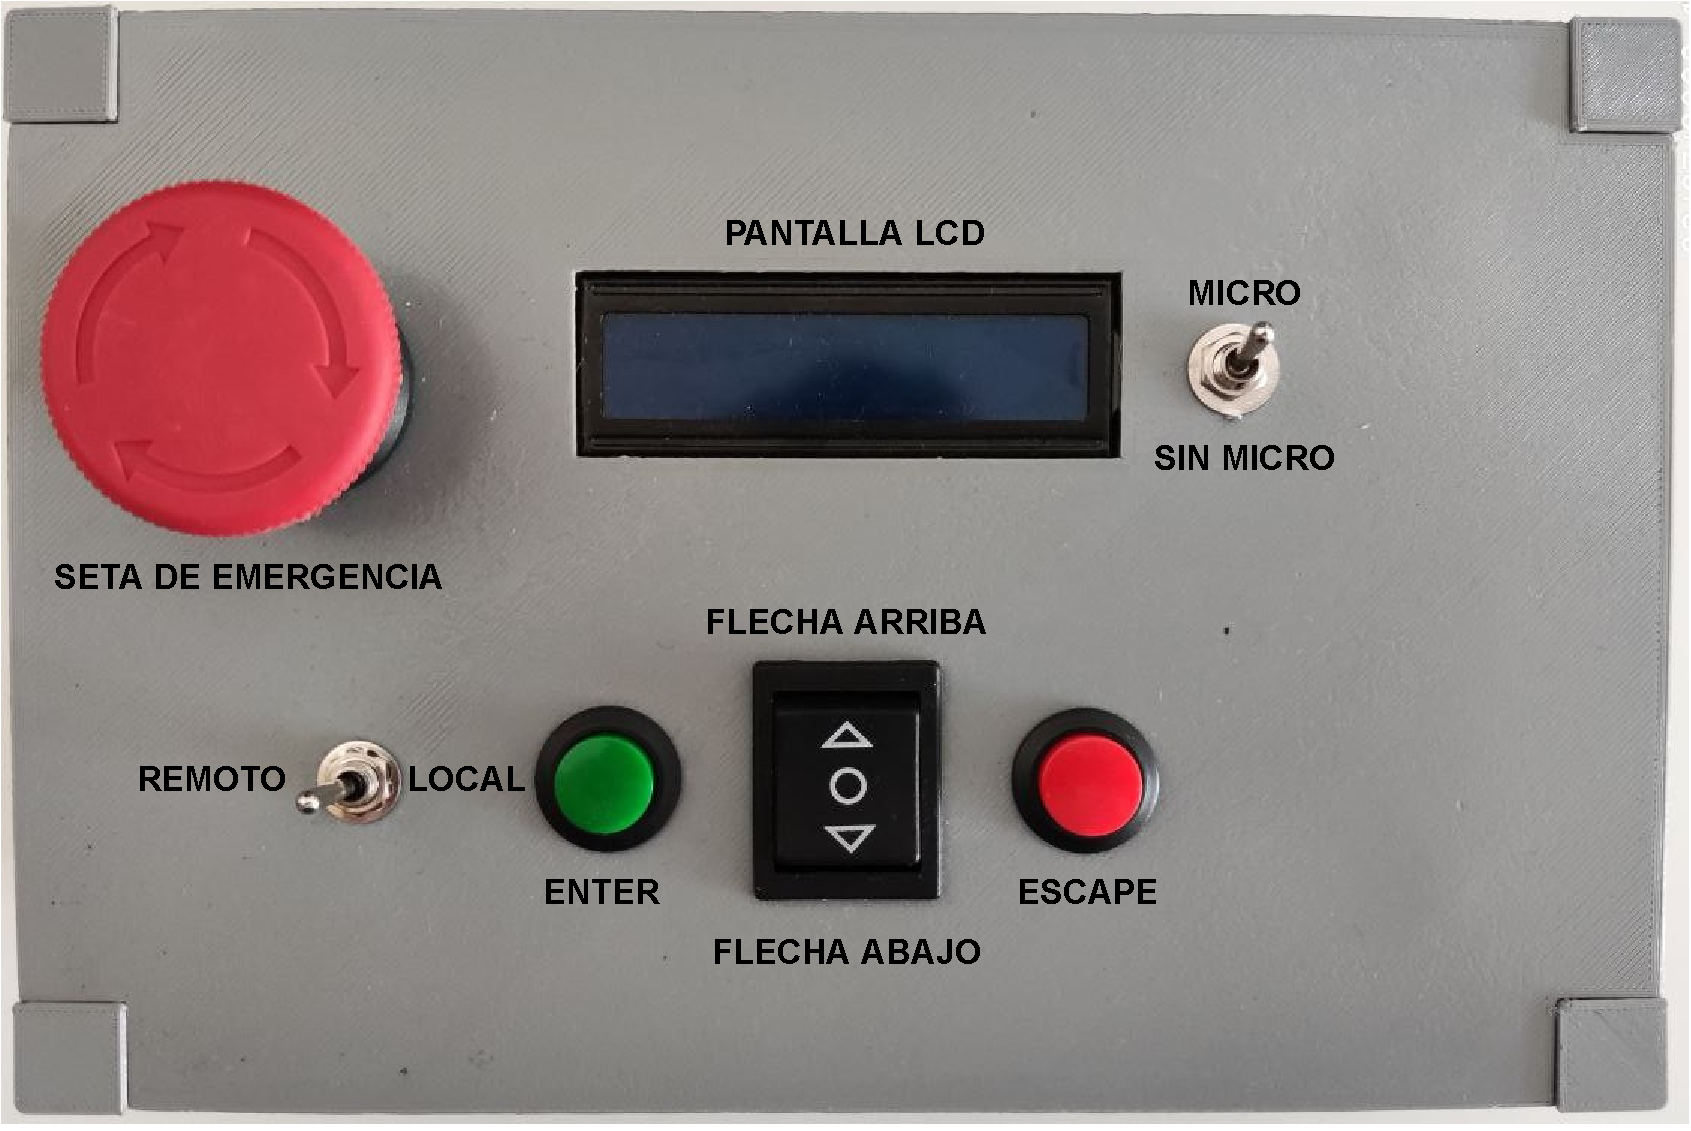
\includegraphics[width=0.75\textwidth]{09-guiadeuso/HMI_REAL.pdf}
	\caption{Comandos del panel de control}
	\label{fig:interfazhmireal}
	\end{figure}

Mediante esta interfaz, el alumno es capaz de mover la cinta transportadora, para ello, debe introducir la posición a la que quiere mover la pieza a a lo largo de la cinta, de esta forma, el panel se comunica con la controladora de los robots ABB para transmitir esa información y realizar la tarea indicada.

La interfaz cuenta con una serie de elementos que permiten el uso de la misma. El panel tiene dos interruptores para seleccionar el modo de uso deseado, con el inferior izquierdo puede seleccionar el uso en modo LOCAL o REMOTO, para escoger indicar la posición de la pieza desde el panel de control de la cinta o desde RobotStudio; y con el superior derecho, puede seleccionar MICRO o SIN MICRO, para activar el microcontrolador o no.

En la pantalla LCD se indica el modo en el que se encuentra el sistema y, además, en modo local se puede visualizar e indicar los datos necesarios para el movimiento de la pieza de forma guiada. Para ello, usando el botón con las flechas puede desplazarse por las diferentes opciones y seleccionar la deseada con el botón ENTER, para retroceder en el menú o salir de él, se debe pulsar el botón ESCAPE.

En la cara trasera (figura \ref{fig:pinesdigitalesreal}) del panel de control se encuentran las conexiones con periféricos:
\begin{itemize}
    \item Conexión Ethernet.
    \item Pines de entrada y salida digital. De izquierda a derecha: RETROCESO, AVANCE, LOCAL, MICRO, EMERGENCIA y FOTO.
    \item Conexiones a los dispositivos integrados en el sistema.
\end{itemize}

    \begin{figure}[htbp]
        \centering
        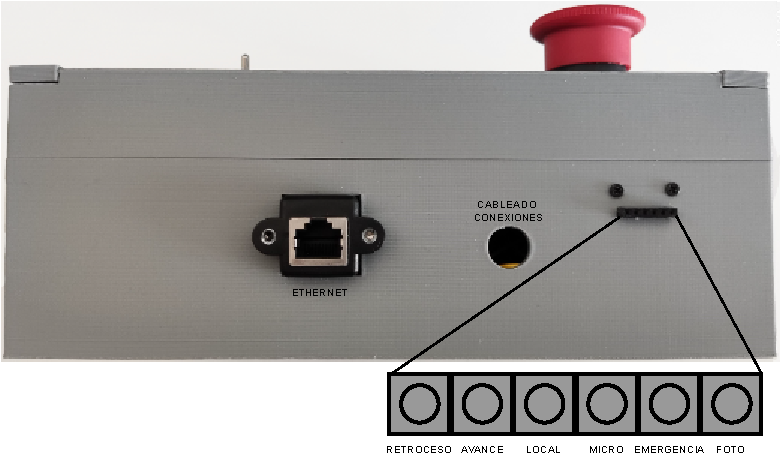
\includegraphics[width=0.75\textwidth]{09-guiadeuso/DIGITALES_REAL.pdf}
        \caption{Conexiones traseras del panel de control}
        \label{fig:pinesdigitalesreal}
        \end{figure}

Mediante la conexión Ethernet se puede comunicar el panel de control con la controladora del robot mediante protocolo TCP/IP. A través de los pines digitales también se puede comunicar la interfaz con la controladora mediante señales digitales. Por un lado, las entradas digitales son los indicadores de los modos LOCAL, MICRO, EMERGENCIA y FOTO. Además, se puede mover la cinta utilizando las salidas digitales RETROCESO y AVANCE en el modo remoto sin microcontrolador.


\section{Tipos de movimiento}

El panel acepta distintas órdenes de movimiento de la cinta. A continuación se comentan las posibilidades con las que se cuenta.

\subsection{Movimiento absoluto}

Este movimiento permite desplazar una pieza a lo largo de la cinta desde el origen de coordenadas de la misma a un punto concreto. La idea para la cual está concebido este tipo de desplazamiento es la colocación de la pieza en el origen de la cinta, lejos del espacio de trabajo del robot, y posicionarla, a continuación, dentro del área de trabajo del robot.

\subsection{Movimiento relativo o discreto}

El movimiento relativo consiste en desplazar la pieza a partir de la posición actual de la misma, por lo que no es necesario tener una referencia exacta de la posición real en la cinta de la pieza. Esto permite avanzar o retroceder una pieza lo deseado independientemente de la posición actual de la misma.

Esto se ve en el momento en que el robot mueve la pieza a lo largo de la cinta la posición, ya que la posición almacenada en el Arduino y la posición real de la pieza dejan de ser coincidentes. Por lo tanto, en caso de volver a depositar la pieza en la cinta y realizar un movimiento se necesita forzosamente utilizar un movimiento relativo para seguir con referencias exactas de la posición de la pieza.

\subsection{Movimiento con actuadores digitales}

De forma alternativa se puede mover la cinta sin control alguno de la posición. Este movimiento se basa simplemente en el avance o retroceso de la cinta accionada digitalmente.

\section{Modos de funcionamiento}

Según la posición de los interruptores de selección el comportamiento del panel y, por ende, de la cinta se modifica.

\subsection{Modo local con microcontrolador}

Los interruptores se colocan en las posiciones  MICRO y LOCAL. En este modo se puede mover la cinta directamente interactuando con los botones y las flechas del panel de control. Se puede avanzar entre los distintos menús y seleccionar entre movimiento absoluto o avance discreto.

En caso de que se necesitase conocer la posición del robot,ésta puede ser conocida El robot también puede recibir la posición en este modo mediante Ethernet utilizando la función leer() (Véase modo remoto con microcontrolador).

\subsection{Modo remoto con microcontrolador}

Los interruptores se colocan en las posiciones MICRO y REMOTO. La controladora es quien envía las órdenes de movimiento mediante protocolo TCP/IP.

Es recomendable partir del código \ref{cod_libreria} que se incluye al final de la guía de uso. Este código se puede utilizar como librería para facilitar el uso del panel de control en modo remoto. Cuenta con tres funciones:
\begin{itemize}
    \item mov\_abs(num distancia). Produce un movimiento absoluto con la posición indicada en milímetros que se le proporciona como entrada numérica.
    \item mov\_dis(num distancia). Produce un avance relativo a la posición actual de la pieza en milímetros que se le proporciona como entrada numérica.
    \item leer(). Lee los datos de estado del sistema, posición y estado del sensor fotoeléctrico. Guarda los datos en las variables “estado”, “posx”, “posy” y “fotoele”.
\end{itemize}

\subsection{Modo local sin microcontrolador}

Los interruptores se colocan en las posiciones SIN MICRO y LOCAL. En este modo se puede accionar la cinta desde las flechas del panel. Permite avanzar y retroceder.

En este modo, a diferencia de los anteriores, es difícil controlar la precisión ya que no se especifican unas coordenadas a las que dirigir la pieza, sino que de forma manual, y mientras se mantenga pulsado la flecha deseada, la pieza se moverá. Esto ocasiona que la única forma en la que el robot pueda conocer la posición aproximada de la pieza sea mediante la señal emitida por el sensor fotoeléctrico.

\subsection{Modo remoto sin microcontrolador}

Los interruptores se colocan en las posiciones SIN MICRO y REMOTO. En este modo se puede accionar la cinta desde la controladora accionando las salidas digitales AVANCE y RETROCESO. Para que la cinta se mueva, es importante que solo sea activada una de las señales. En caso de que ambas sean activadas, la cinta no se moverá y se bloqueará hasta que una de las dos se anule.

A nivel digital, este modo funciona con las mismas señales que el anterior, por lo que tendrá un funcionamiento similar; mientras se reciba la señal de avance o retroceso, la cinta se moverá, pero en este caso, no se puede especificar una coordenada concreta a la que enviar la pieza. La forma de posicionar la pieza es mediante el sensor fotoeléctrico, cuya señal digital puede ser leída por parte de la controladora mediante el pin especificado para ello.

\subsection{Modo emergencia}

Para acceder a este modo se tiene que presionar la seta de emergencia. En este modo el sistema queda bloqueado y la cinta deja de moverse a modo de seguridad. Para que el panel de control vuelva a un estado utilizable hay que desarmar la seta de emergencia.

\begin{lstlisting}[language=,caption={Librería}, breaklines=true, label=cod_micro]
    MODULE Module1  
        !Declaración de variables del programa
        !Objeto de socket de conexión
        VAR socketdev my_socket;
    
        !Variable de estado
        VAR string estado:=0;
    
        !Cadenas de caracteres de recepción
        VAR rawbytes receive_string;
        VAR string string1;
        VAR string posx_str;
        VAR string posy_str;
        VAR string fotoele_str;
    
        !Posiciones de los datos a lo largo de la cadena recibida
        VAR num xpos;
        VAR num ypos;
        VAR num fepos;
        
        !Valores numéricos finales recibidos
        VAR num posx;
        VAR num posy;
        VAR byte fotoele;
        
        !Comprobación de recepción correcta
        VAR bool okposx:=true;
        VAR bool okposy:=true;
            
        !Función de apertura de socket
        PROC abricomunicacion()        
            SocketCreate my_socket; !crea el socket
            SocketConnect my_socket, "192.168.50.200", 4012;        
        ENDPROC
        
        !Función de lectura de estado y 
        PROC leer()
            !Se abre el socket y conecta al Arduino
            abricomunicacion;
            
            !Escribe en el socket la cadena "STATUS" para que el Arduino envíe sus datos
            SocketSend my_socket,\Str:="STATUS"; 
            WaitTime 0.1; !espera un tiempo
    
            !Recibe la respuesta 
            ClearRawBytes receive_string;
            SocketReceive my_socket \RawData := receive_string,\Time:=WAIT_MAX;
            
            !Desempaqueta los bytes y los convierte en una cadena de caracteres
            UnpackRawBytes receive_string, 1, string1 \ASCII:=32;
            
            !Se buscan las posiciones de cada variable a lo largo de la cadena
            xpos        := StrFind(string1, 1, "=");
            ypos        := StrFind(string1, xpos+1, "=");
            fepos       := StrFind(string1, ypos+1, "=");
            
            !Se trocea la cadena para obtener subcadenas con los datos recibidos
            estado      := StrPart(string1, 0, 1);
            posx_str    := StrPart(string1, xpos+1, ypos - xpos - 3);
            posy_str    := StrPart(string1, ypos+1, fepos - ypos - 3);
            fotoele_str := StrPart(string1, fepos+1, 1);
    
            !Se transforman las cadenas a los tipos de datos que les corresponden
            okposx      :=  StrToVal(posx_str,posx);
            okposy      :=  StrToVal(posy_str,posy);
            fotoele     :=  StrToByte(fotoele_str);
            
            !Conversión de pulsos a milímetros
            posx := posx / 100;
    
            !Se cierra el socket
            ClearRawBytes receive_string;
            SocketClose my_socket;
        ENDPROC
    
        !Funciones de movimiento. Se envía una cadena con un caracter y la distancia a recorrer. Si el carácter es "M", el movimiento es absoluto, mientras que si es "R" es relativo.
        PROC mov_abs(num distancia)
            abricomunicacion;
            SocketSend my_socket,\Str:="M;X=" + ValToStr(distancia*100) + ";";
            WaitTime 0.1;
            SocketClose my_socket;
        ENDPROC
        
        PROC mov_dis(num distancia)
            abricomunicacion;
            SocketSend my_socket,\Str:="R;X=" + ValToStr(distancia*100) + ";";
            WaitTime 0.1;
            SocketClose my_socket;
        ENDPROC

        !Bucle principal del programa
        PROC main()
            !Se cierran los posibles sockets abiertos
            SocketClose my_socket;
            
            !Aquí empieza el programa del alumno
            !
        ENDPROC
    ENDMODULE
\end{lstlisting}



